\documentclass[../main.tex]{subfiles}

\begin{document}
\chapter{Progress since May 2020}\label{progress}
Note - main literature review has been excluded from this report as it was submitted last year but it will be included in my final thesis.
My progress since May 2020 is summarised and then my thesis layout excluding the main introduction with some sections filled in is included.

\textbf{Background}
Over thousands of years crops have been domesticated to fix desirable traits.
A side effect of this is that genetic bottlenecks have reduced variation over time \autocite{tanksleySeedBanksMolecular1997}.
Many crop\hyp{}improvement methods aim to increase diversity.
For example, mutagenesis and marker assisted breeding generate variation over the whole genome, following which desirable phenotypes are selected for and then back\hyp{}crossed to remove undesired mutations \autocite{tuberosaMarkerAssistedbreedingBreedSee2012}.
An advantage is that an understanding of the genes involved is unnecessary, but it can take many years over many plant generations to breed traits into elite lines.
Transgenesis and genome engineering methods such as CRISPR are much more specific, only editing genes of interest.
A background understanding of which genes to edit is necessary but these methods are much faster and engineering of elite lines directly may be possible \autocite{sedeekPlantGenomeEngineering2019}.

Most genome editing to date has focussed on mutating coding sequences (CDSs).
For example, Gn1a regulates the number of reproductive organs in rice, and GS3 regulates grain size.
Mutations in \textit{GS3} and \textit{Gn1a} coding sequences lead to an increase in grain size and grain number \autocite{shenQTLEditingConfers2018}.
In the cucumber, the translation initiation factor eIF4E translates the RNA of several viruses.
Loss of function of this gene confers virus resistance \autocite{chandrasekaranDevelopmentBroadVirus2016}.
In the tomato, LBD40 has a role in lateral organ development and jasmonate signalling.
Loss of function of this gene resulted in increased drought tolerance \autocite{liuCRISPRCas9Targeted2020}.

Engineering of \textit{cis}\hyp{}regulatory regions is an emerging strategy.
Compared to mutations in coding sequences that alter protein structure, \textit{cis}\hyp{}regulatory variants are often less pleiotropic and cause subtle phenotypic changes by modifying the pattern, timing or strength of gene expression \autocite{wittkoppCisregulatoryElementsMolecular2012}.
The rice \textit{SWEET14} gene codes for a sucrose transporter, and is also susceptible to bacterial blight.
Disruption of the CDS confers blight resistance but plants have reduced growth as they lose function of the sugar transporter.
4 bp and 9 bp deletions in the \textit{SWEET14} promoter conferred blight resistance without significantly affecting plant growth \autocite{liHighefficiencyTALENbasedGene2012}.
The CLAVATA-WUSCHEL feedback signalling pathway controls meristem size \autocite{somssichCLAVATAWUSCHELSignalingShoot2016}.
WUS is expressed in the organising centre of the meristem where it increases the expression of the secreted peptide CLV3.
CLV3 binds to the receptor CLV1 which represses \textit{WUS} expression.
In tomato, mutations in the \textit{CLV3} and \textit{WUS} promoters increased the locule number and fruit size due to stem cell overproliferation \autocite{rodriguez-lealEngineeringQuantitativeTrait2017}.
Recently, the promoter of the \textit{CLV3} orthologue \textit{CLE7} in maize was mutated \autocite{liuEnhancingGrainyieldrelatedTraits2021}.
Several mutations increased grain yield, while one mutation decreased grain yield.

In my project I will be using genome engineering approaches to add variation into \textit{Arabidopsis thaliana} as it is a model plant with lots of data already published.
Specifically, I will engineer genes in the nitrogen\hyp{}response network.
The nitrogen cycle is one of the most important biogeochemical cycles on earth \autocite{lehnertReversingNitrogenFixation2018}.
Atmospheric nitrogen is converted to ammonium by nitrogen fixing bacteria in symbiosis with plants (e.g., Rhizobium \autocite{molingEvolutionRhizobiumNodulation2015}) and free\hyp{}living bacteria in the soil (e.g., Azotobacter \autocite{bhattacharyyaPlantGrowthpromotingRhizobacteria2012}).
Ammonium is then converted to nitrite then nitrate by nitrifying bacteria.
Both ammonium and nitrate are readily absorbed by plant roots.
Nitrogen is often the most limiting essential nutrient for crop growth.
Crops developed during the Green Revolution were bred specifically to respond to fertilisers and increase yields.
Problems with overuse of fertiliser include the release of the greenhouse gases nitrous oxide from the soil \autocite{zumftCellBiologyMolecular1997} and carbon dioxide from production of the fertiliser.
Soluble ions such as nitrate are washed into water ways causing eutrophication \autocite{gallowayChronologyHumanUnderstanding2013}.
N fertiliser is inaccessible to farmers in developing regions due to the price and disrupted supply chains.
It is desirable to increase the N\hyp{}use efficiency of crops to reduce the dependency on nitrogen fertilisers.

Changes in N impact many plant traits such as growth and development, lateral roots, root depth, rosette size and flowering time \autocite{abalosPlantTraitbasedApproaches2019,castromarinNitrateRegulatesFloral2011}.
These traits are the result of large\hyp{}scale transcriptional change.
Recent systems biology approaches have identified a subnetwork of candidate TFs coordinating these changes \autocite{gaudinierTranscriptionalRegulationNitrogenassociated2018,varalaTemporalTranscriptionalLogic2018} (\autoref{fig:n-subnetwork}).

\begin{figure}[hbt!]
	\begin{center}
		\capstart
		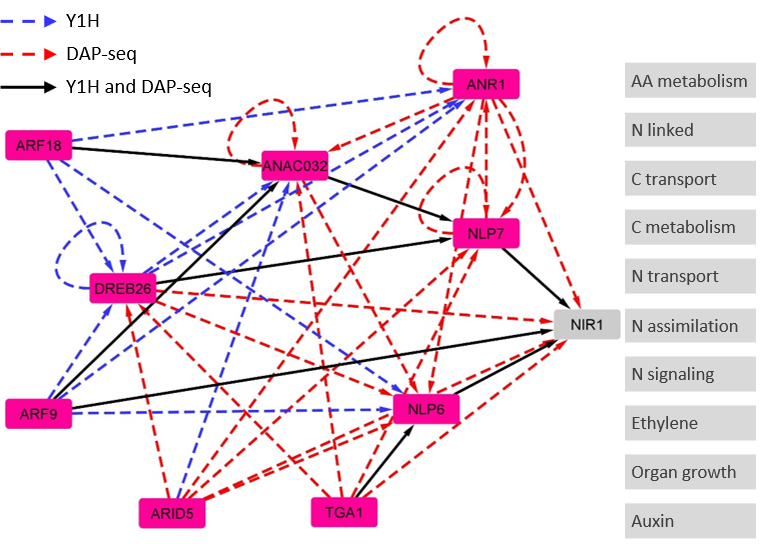
\includegraphics[width=0.8\columnwidth]{validate_edges/Nsubnetwork}
		\caption{
			\textbf{Nitrate\hyp{}response subnetwork}
			The nitrate\hyp{}response subnetwork built using yeast one\hyp{}hybrid (Y1H) \autocite{gaudinierTranscriptionalRegulationNitrogenassociated2018} and DNA affinity purification sequencing (DAP-seq) \autocite{omalleyCistromeEpicistromeFeatures2016} data.
            Nodes (TFs) are in pink.
            Edges are represented by blue (supported by Y1H data) and red (supported by DAP-seq data) dotted lines and black solid lines (supported by both DAP-seq and Y1H data).
            NIR1 is an important target gene involded in nitrite reductase and is a useful transcriptional output gene for measuring the plant nitrate response.
            The master regulators in the subnetwork coordinate many pathways in response to nitrate (grey boxes).
			\label{fig:n-subnetwork}
		}
	\end{center}
\end{figure}

The predicted edges in the subnetwork form several feed\hyp{}forward loops (FFLs).
The subnetwork is predicted to coordinate responses of many downstream genes.
NLP7 and TGA1 knockouts no longer grow lateral roots in response to N, and downstream genes no longer change expression in response to N.
This is also expected to be true for ARF18 and ARF9 \autocite{gaudinierTranscriptionalRegulationNitrogenassociated2018}.
Loss of function of these master regulators individually and in combination will disrupt plant responses to N.
We would like to validate connections in the network so that we understand the role of network motifs (e.g., FFLs) in regulating responses to changes in nitrate.
This will enable us to rationally and predictably engineer the subnetwork to improve the nitrogen use\hyp{}efficiency.

\textbf{Adding novel genetic variation to promoter regions to disrupt edges}
Four nitrogen master regulators were identified. \textasciitilde{}500 bp open chromatin regions in each promoter were identified. These regions were scanned for SpCas9 PAMs sites. 122 guides were designed ensuring predicted on-target efficiency of \textgreater{} \SI{40}{\percent}, with \textasciitilde{}30 guides per promoter. A custom Python script allocated each guide into a pair 90-110 bp apart with the aim of increasing the variety of mutations, with a chance to cause a large deletion between the two PAM sites in a pair. 122 sgRNA cassettes were constructed and used to build 96 final Cas9 constructs each containing a guide pair using Golden Gate assembly. 96 strains of Agrobacteria were transformed with the plasmids. These strains were combined equally and then sprayed onto ~100 Col-0 Arabidopsis thaliana plants using the Agrobacterium-mediated floral dip method. Seeds were collected, grown on selectable kanamycin media and 200 T1 lines were transferred to soil. These plants have now been bagged ready for seed collection. Leaf samples of the T1 lines have been stored at \SI{-70}{\degreeCelsius}. In the future 500 T2 lines will be grown and genotyped using a CRISPR sequencing approach. Plants containing a range of variation in the promoter regions of interest will be grown to T3 level for phenotyping and expression analysis using RNA-seq.

\textbf{Adding network motifs to the N subnetwork}
Another aim is to add genetic feedback into the N subnetwork to influence expression dynamics, promoting bistability, efficient switching behaviour, robustness in the presence of noise, and tunability. NLP7 is regulated by ARF18 through ANAC032 (\autoref{fig:n-subnetwork}). To add genetic feedback from NLP7 to ARF18, a synthetic promoter responding only to NLP7 controlling a synthetic TF which binds to and regulates ARF18 is desired. To design synthetic promoters, more information is needed about promoter architecture. To this aim, a comprehensive bioinformatics analysis was undertaken to elucidate the complex promoter architectural differences between constitutive and variable genes, and tissue-specific and non-specific genes.

\textbf{Understanding promoter architecture to allow engineering of synthetic promoters}
Tissue-specific and non-specific promoter categories were added to the previous promoter architecture analysis using Tau tissue-specificity ranking because the coefficient of variation of expression ranking excluded tissue-specific genes. Promoters were scanned using a sliding window approach to identify regions of importance for explaining differences in expression between the gene categories. A 400 bp region upstream from the ATG start codon was chosen and statistically analysed. A significant difference in TFBS percent coverage was found between groups in the 400 bp promoter region. In the same region GC content was higher in constitutive promoters than variable, and higher in non-specific than tissue-specific promoters. TATA boxes were enriched in variable promoters compared to the background, and negatively enriched in constitutive promoters compared to the background.
For engineering synthetic promoters the region closest to TSS/start codon is more important as differences here explain the different expression patterns of the different gene categories. TATA boxes should be included in responsive promoters. Promoters with more open chromatin are more actively expressed, and motifs falling within open chromatin are more important. This was useful to know for the CRISPR library approach, where only variation was added to promoter regions falling within open chromatin to ensure important regions were disrupted.

\textbf{Adding synthetic genetic feedback to the N subnetwork}
Several different synthetic N-responsive promoters were designed and assembled. These respond to either NLP7, TGA1, bZIP3 (activators) or HHO2 (repressor). Promoters with combinations of NLP7 and TGA1 or NLP7 and bZIP3 were also assembled. The response of these promoters to the TFs that bind them was tested in Arabidopsis leaf protoplasts using a dual luciferase assay. These experiments will be repeated using the same batch of plants as variation was high between batches. In the near future the synthetic TFs will be assembled and tested in protoplasts using qPCR, to make sure they activate or repress ARF18 as designed. Once all parts have been tested, the synthetic genetic feedback circuit will be constructed, with the synthetic promoter controlling the synthetic TF which then activates or represses ARF18. Transcriptomics of important N master regulators will be tested transiently in protoplasts using qPCR. The circuit will also be tested in stable lines where expression and phenotype analysis will be conducted.

\textbf{Timeline}

Planned work over the next year is shown in \autoref{fig:gantt}.
\begin{sidewaysfigure}[hbt!]
	\begin{center}
		\capstart
		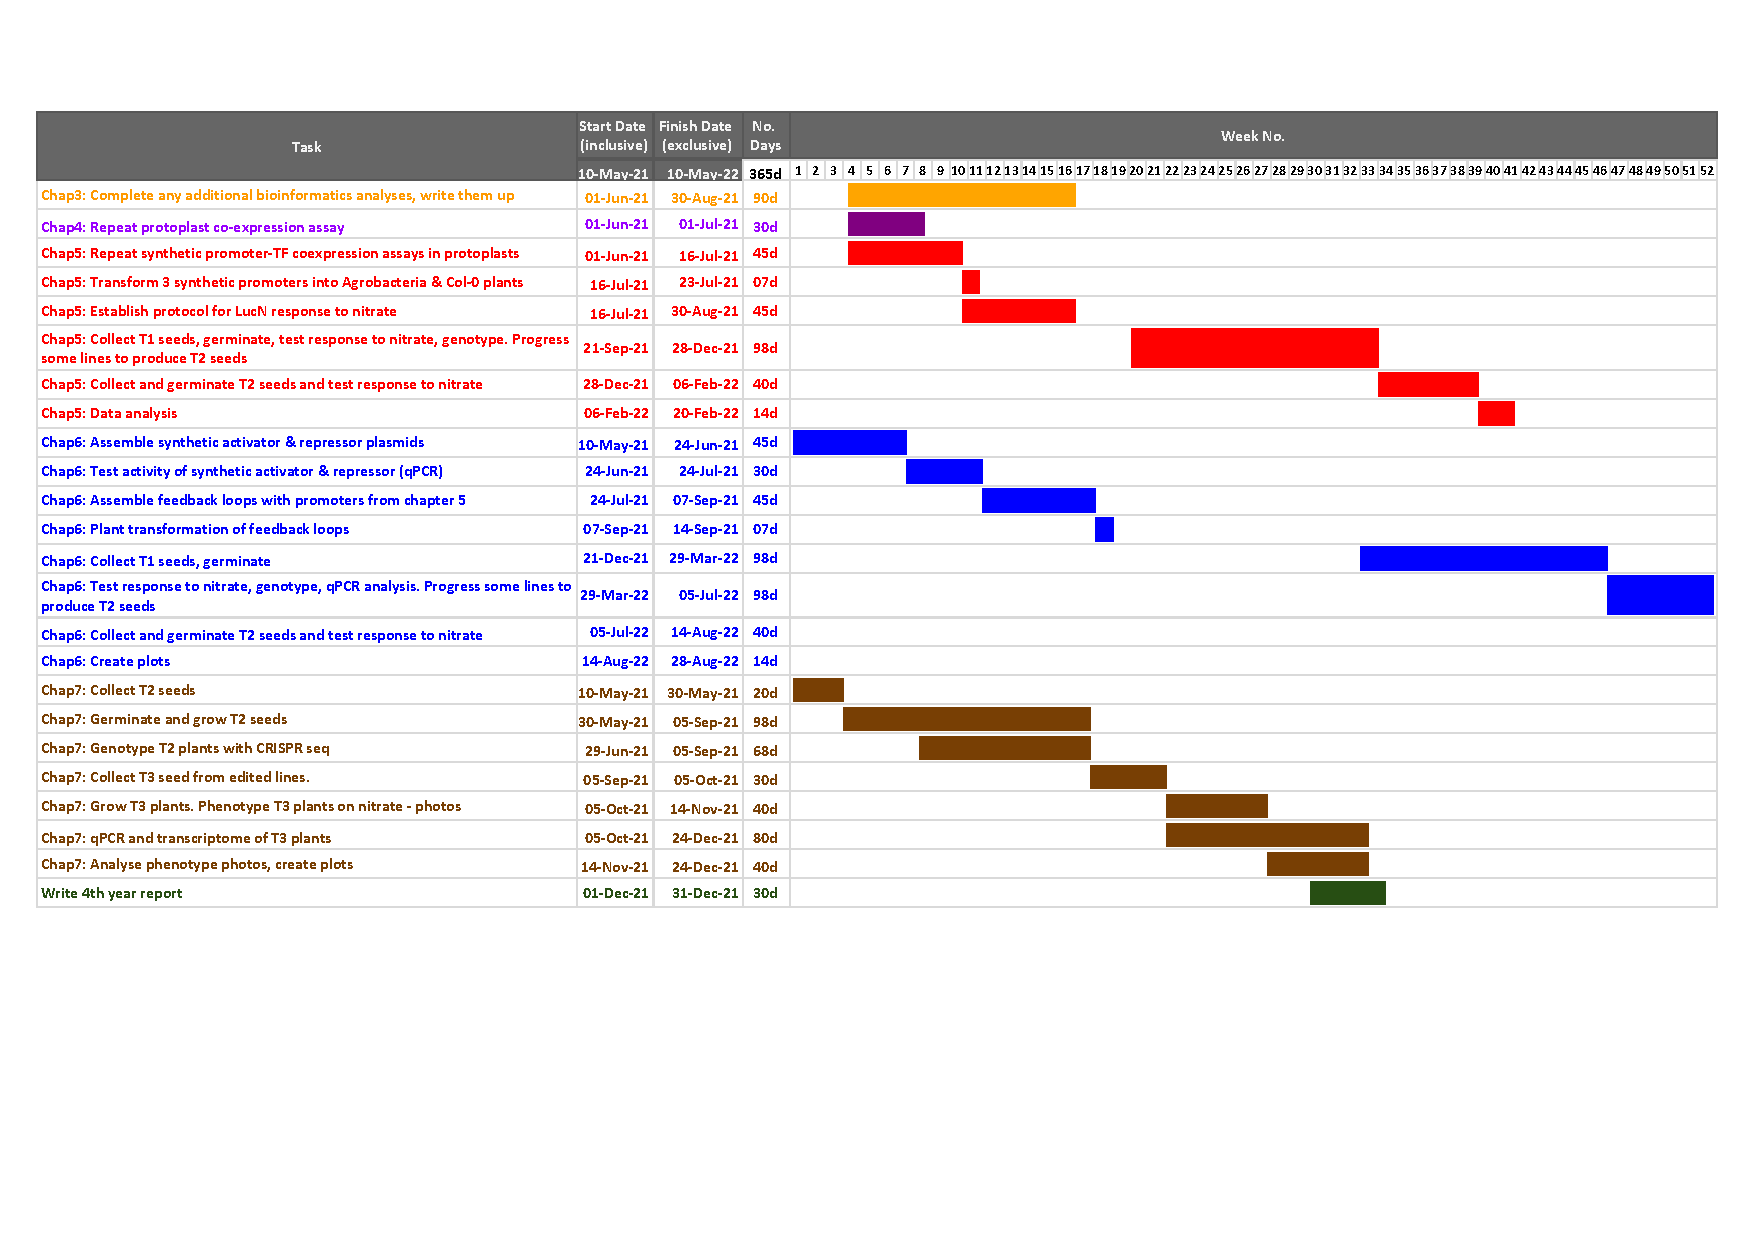
\includegraphics[width=1\columnwidth]{gantt_charts/2021ProgressReviewTimeline}
		\caption{
			\textbf{Timeline}
			Planned work for each of the thesis chapters is colour coded.            
			\label{fig:gantt}
		}
	\end{center}
\end{sidewaysfigure}